\newpage
\section{Comprobamos qué tipo de arranque tiene la placa}

\begin{center}
\vspace{5mm}
 
 
 \begin{tcolorbox}[title=Comprobamos qué tipo de arranque tiene la placa]
    \orden{ls /sys/firmware/efi/efivars}
 \end{tcolorbox}
 
 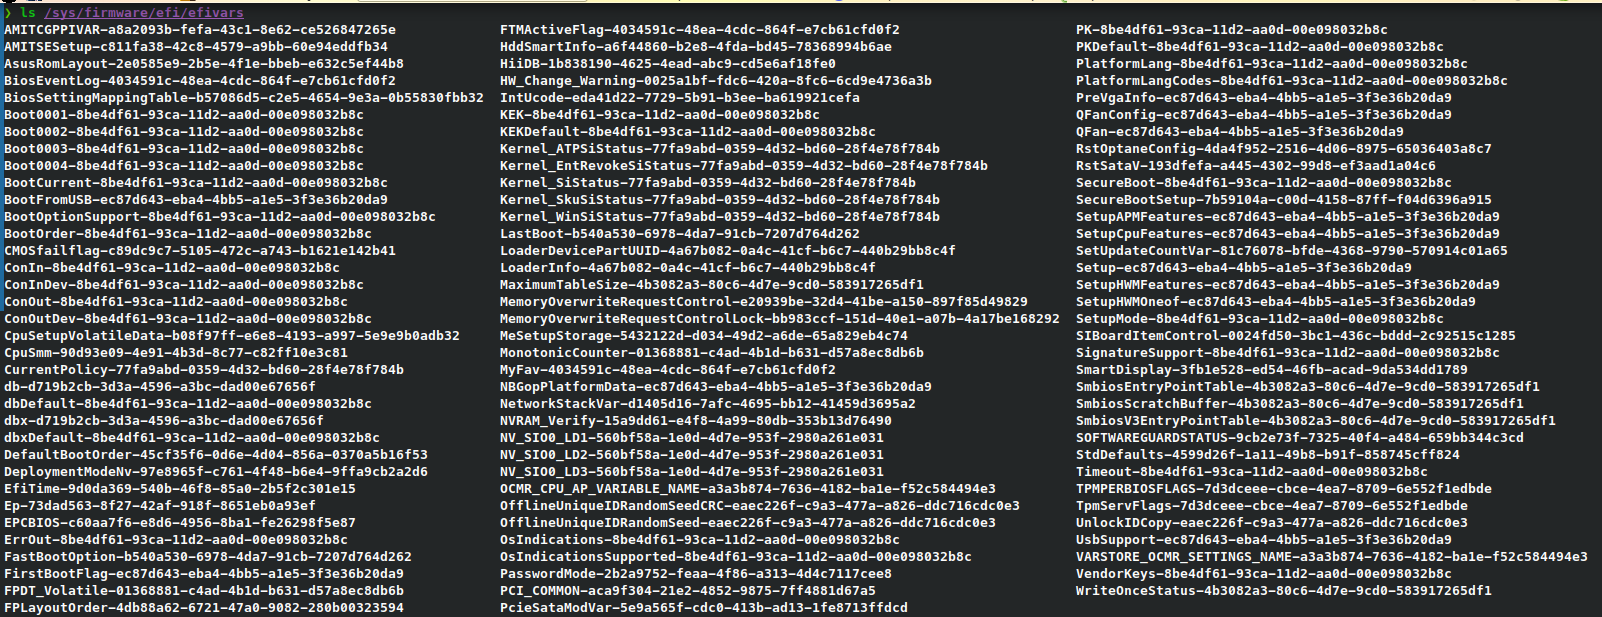
\includegraphics[width=.95\textwidth]{3 UEFI.png}\\
\end{center}

 \vspace{15mm}

 \begin{tcolorbox}[title=Si  vemos  esta  salida\,  entonces  es  un  arranque  \btrojo{UEFI}]
Instalaremos el paquete \tazul{grub} y, adicionalmente, \tazul{efibootmgr}.
 \end{tcolorbox}

 \vspace{15mm}

 \begin{tcolorbox}[title=Si  no la vemos entonces  es  un arranque  \brojo{BIOS}]
Instalaremos únicamente el paquete \tazul{grub}.
 \end{tcolorbox}
 \newpage
